%----------------------------------------------------------------------------------------
%	PACKAGES AND OTHER DOCUMENT CONFIGURATIONS
%----------------------------------------------------------------------------------------

\documentclass[12pt]{article}
\usepackage{graphicx}
\usepackage[utf8]{inputenc}  
\usepackage[T1]{fontenc} 
\usepackage[top=1.5cm,bottom=1.5cm,left=1.3cm,right=1cm,asymmetric]{geometry}

\usepackage{amsfonts}
\usepackage{graphicx}
\usepackage{amsmath}
\usepackage{fancyhdr}
\usepackage{array,multirow,makecell}
\usepackage{cancel}
\usepackage{subfig}
\usepackage{wrapfig}
\setcellgapes{1pt}
\makegapedcells
\newcolumntype{R}[1]{>{\raggedleft\arraybackslash }b{#1}}
\newcolumntype{L}[1]{>{\raggedright\arraybackslash }b{#1}}
\newcolumntype{C}[1]{>{\centering\arraybackslash }b{#1}}


\usepackage{tikz}
\usetikzlibrary{arrows,automata,fit}

\pagestyle{fancy}
\renewcommand{\footrulewidth}{1pt}
\fancyhead[R]{\textit{Master MVA : Probabilistic graphical models}}
\fancyfoot[L]{\textit{}}
%\usepackage{unicode-math}
%\setmathfont{XITS Math}
%\setmathfont[version=setB,StylisticSet=1]{XITS Math}


%\geometry{hmargin=1.5cm,vmargin=2cm}   

\begin{document}
\section*{Latent dirichlet allocation for label modelling}
\section*{Thibaud Ehret \& Sammy Khalife}
\begin{figure}[!h]
\centering
\captionsetup{justification=centering,margin=2cm}
\includegraphics[width=15cm]{LDA.png}
\caption{Graphical model associated to LDA model}
\end{figure}
\begin{figure}[!H]
	\centering
	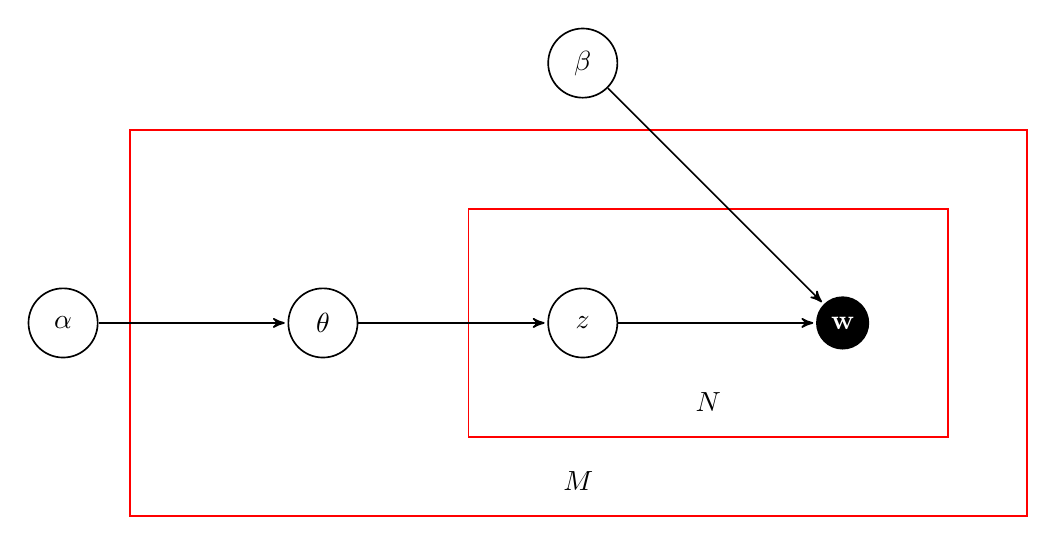
\begin{tikzpicture}[->,>=stealth',shorten >=1pt,auto,node distance=3.3cm,
		semithick]
		\tikzstyle{every state}=[fill=white,draw=black,text=black]
		\tikzstyle{final}=[circle, fill=black,draw=black,text=white]
		\node[state]         (A)                    {$\alpha$};
		\node[state]         (B) [right of=A]       {$\theta$};
		\node[state]         (C) [right of=B]       {$z$};
		\node[state]         (D) [above of=C]       {$\beta$};
		\node[final]         (E) [right of=C]       {$\textbf{w}$};
		\node (B1) [draw=red, fit= (E) (B) (C) , inner sep=2cm] {};
		\node (B2) [draw=red, fit= (C) (E), inner sep=1cm] {};
		\node [yshift=3.0ex, black] at (B1.south) {$M$};
		\node [yshift=3.0ex, black] at (B2.south) {$N$};
		\path (A) edge              (B)
	              (C) edge              (E)
	              (D) edge              (E)
	              (B) edge              (C);
	\end{tikzpicture}
	\caption{LDA model}
	\label{LDA_model}
\end{figure}


\begin{eqnarray*}
p(\textbf{w}|\alpha, \beta) &  = & \int p(\theta | \alpha, \beta)p(\textbf{w} | \alpha, \beta, \theta)d\theta\\
\end{eqnarray*}
In the LDA model, we have $ \theta \perp \beta$, and $p(w_{i} | \alpha, \beta, \theta) \perp p(w_{j} | \alpha, \beta, \theta)$  for $ i \neq j $
\begin{eqnarray*}
p(\textbf{w}|\alpha, \beta) & = & \int p(\theta | \alpha) \prod_{n=1}^{N} p(\textbf{w}_{n} | \alpha, \beta, \theta)d\theta\\
& = & \int  p(\theta |\alpha) \prod_{n=1}^{N}  \sum_{z_{n}}p(z_{n}|\alpha, \beta, \theta)p(\textbf{w}_{n} | \alpha, \beta, \theta, z_{n}) d\theta\\
\end{eqnarray*}
Moreover $z \perp (\alpha,\beta)$ and $\textbf{w}_{n} \perp (\alpha,\theta)$,
\begin{eqnarray*}
p(\textbf{w}|\alpha, \beta) & = & \int p(\theta | \alpha)  \prod_{n=1}^{N}  \sum_{z_{n}}p(z_{n} |\theta)p(\textbf{w}_{n} | z_{n}, \beta) d\theta\\
\end{eqnarray*}









\section{The algorithm}
We saw the complexity of the distribution associated to this model, therefore one can not simply calculate the posterior distribution for the inference and the parameter estimation. We will briefly present the algorithm used to calculate the inference and an approximation of the parameters. However, even if the distribution can not be computed, the algorithm is based on the EM principle.

\subsection{Inference}

The trick to be able to calculate the inference for the LDA model to calculate the variational inference which is a lower bound but easily calculable.

The lower bound is computed using the simplified graphical model presented in figure \ref{low_bound_model} which does not have the coupling between $\theta$ and $\beta$ and $\textbf{w}$.

The parameters $\gamma$ and $\phi$ for this new model are estimated by minimmizing the Kullback-Leibler divergence which has been shown to be good lower bound for the log-likelyhood. These are the parameters that we will use in the next part in order to estimate the parameters. 

\subsection{Parameter estimation}

We uses a modified version of the EM algorithm for this part. The expectation part, also called E-step, consists in computed the best variational parameters $\gamma$ and $\phi$ for the lower bound presented in the previous section. The maximization part, M-step, consists in optimizing the model parameter $\alpha$ and $\beta$ with the variational parameter fixed.
Just like in the EM algorithm, both step are then iterated until the bound of the model \ref{low_bound_model} converges.

\begin{figure}
	\centering
	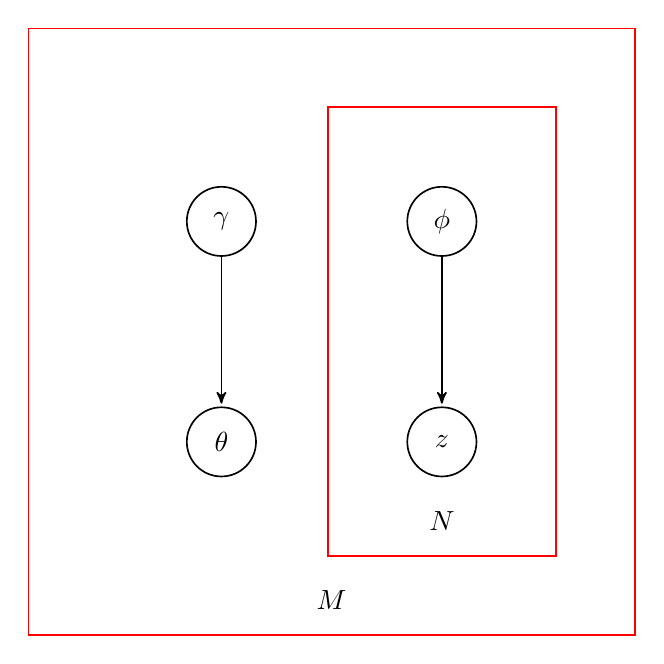
\begin{tikzpicture}[->,>=stealth',shorten >=1pt,auto,node distance=2.8cm,
		semithick]
		\tikzstyle{every state}=[fill=white,draw=black,text=black]
		\node[state]         (A)                    {$\gamma$};
		\node [state]        (B) [below of=A]       {$\theta$};
		\node[state]         (C) [right of=A]       {$\phi$};
		\node[state]         (D) [below of=C]       {$z$};
		\node (B1) [draw=red, fit= (A) (B) (C) (D), inner sep=2cm] {};
		\node (B2) [draw=red, fit= (D) (C), inner sep=1cm] {};
		\node [yshift=3.0ex, black] at (B1.south) {$M$};
		\node [yshift=3.0ex, black] at (B2.south) {$N$};
		\path (A) edge              (B)
	              (C) edge              (D);
	\end{tikzpicture}
	\caption{Graphical model used to calculate the lower bound of the log-likelyhood for the LDA graphical model}
	\label{low_bound_model}
\end{figure}

\end{document}
